\documentclass{article}
\usepackage[english,russian]{babel}
\usepackage{textcomp}
\usepackage{geometry}
  \geometry{left=2cm}
  \geometry{right=1.5cm}
  \geometry{top=1.5cm}
  \geometry{bottom=2cm}
\usepackage{tikz}
\usepackage{multicol}
\usepackage{hyperref}
\usepackage{listings}
\pagenumbering{gobble}

\lstdefinestyle{csMiptCppStyle}{
  language=C++,
  basicstyle=\linespread{1.1}\ttfamily,
  columns=fixed,
  fontadjust=true,
  basewidth=0.5em,
  keywordstyle=\color{blue}\bfseries,
  commentstyle=\color{gray},
  texcl=true,
  stringstyle=\ttfamily\color{orange!50!black},
  showstringspaces=false,
  numbersep=5pt,
  numberstyle=\tiny\color{black},
  numberfirstline=true,
  stepnumber=1,      
  numbersep=10pt,
  backgroundcolor=\color{white},
  showstringspaces=false,
  captionpos=b,
  breaklines=true
  breakatwhitespace=true,
  xleftmargin=.2in,
  extendedchars=\true,
  keepspaces = true,
  tabsize=4,
  upquote=true,
}


\lstdefinestyle{csMiptCppLinesStyle}{
  style=csMiptCppStyle,
  frame=lines,
}

\lstdefinestyle{csMiptCppBorderStyle}{
  style=csMiptCppStyle,
  framexleftmargin=5mm, 
  frame=shadowbox, 
  rulesepcolor=\color{gray}
}

\lstset{style=csMiptCppLinesStyle}
\lstset{literate={~}{{\raisebox{0.5ex}{\texttildelow}}}{1}}


\renewcommand{\thesection}{\arabic{section}}
\makeatletter
\def\@seccntformat#1{\@ifundefined{#1@cntformat}%
   {\csname the#1\endcsname\quad}%    default
   {\csname #1@cntformat\endcsname}}% enable individual control
\newcommand\section@cntformat{Часть \thesection:\space}
\makeatother



\begin{document}
\title{Семинар \#1: Библиотека SFML.\vspace{-5ex}}\date{}\maketitle


\section{Подключение библиотеки SFML}
Библиотека SFML (Simple and Fast Multimedia Library) - простая и быстрая библиотека для работы с мультимедиа. Кроссплатформенная (т. е. одна программа будет работать на операционных системах Linux, Windows и MacOS). Позволяет создавать окно, рисовать в 2D и 3D, проигрывать музыку и передавать информацию по сети. 

\subsection*{Подключение библиотеки на Windows с использованием пакетного менеджера MSYS2}
Самый простой способ установки библиотеки на компьютер -- это использованием пакетного менеджера. В данном руководстве будет рассматриваться установка библиотеки с помощью пакетного менеджера \texttt{pacman} среды MSYS2. Для того, чтобы установить SFML в среде MSYS2 проделайте следующее:
\begin{enumerate}
\item Найдите как называется пакет SFML в среде MSYS2. Для этого просто загуглите \texttt{msys2 install sfml} и одной из первых ссылок должен быть страница библиотеки SFML сайта \texttt{packages.msys2.org}. Зайдите на эту страницу и найдите команду для установки SFML. Скопируйте эту команду. Это может быть команда:
\begin{verbatim}
    pacman -S mingw-w64-x86_64-sfml
\end{verbatim}
или просто
\begin{verbatim}
    pacman -S sfml
\end{verbatim}
\item Откройте терминал MSYS2 для установки пакетов. Если у вас установлен MSYS2, то это можно сделать, нажав Пуск и начав печатать "MSYS2". Вставьте команду для установки SFML в терминал и нажмите Enter. Возможно потребуется нажать клавишу \texttt{Y} и Enter, чтобы подтвердить установку. После этого библиотека установится на компьютер. 

\item Убедитесь, что библиотека установилась. Для этого перейдите в папку, где установлен MSYS2, по умолчанию это \texttt{C:\textbackslash msys64}. После этого найдите папку в которой установилась библиотека SFML. Если вы используете 64-х битную версию компилятора MinGW, то библиотека установится в папке \texttt{C:\textbackslash msys64\textbackslash mingw64}. В папке \texttt{C:\textbackslash msys64\textbackslash mingw64\textbackslash bin} должны лежать \texttt{.dll} файлы библиотеки SFML. А в папке \\ \texttt{C:\textbackslash msys64\textbackslash mingw64\textbackslash include} -- заголовочные файлы библиотеки.

\item Убедитесь, что путь до папки, в которой лежат \texttt{.dll} файлы библиотеки SFML прописан в переменной среды \texttt{PATH}. Если этого пути в переменной \texttt{PATH} нет, то добавьте его.

\item Если терминал был открыт, то закройте его, а потом откройте заново.
\end{enumerate}
Всё, библиотека установлена. Теперь можно компилировать файл исходного кода, использующий библиотеку SFML следующим образом:
\begin{verbatim}
    g++ main.cpp -lsfml-graphics -lsfml-window -lsfml-system
\end{verbatim}



\subsection*{Подключение библиотеки на Linux с использованием пакетного менеджера}
Нужно установить SFML с помощью стандартного пакетного менеджера. Предположим, что используется пакетный менеджер \texttt{apt}:
\begin{verbatim}
    sudo apt install libsfml-dev
\end{verbatim}
Всё, библиотека установлена. Теперь  можно компилировать файл исходного кода, использующий библиотеку SFML следующим образом:
\begin{verbatim}
    g++ main.cpp -lsfml-graphics -lsfml-window -lsfml-system
\end{verbatim}



\subsection*{Тестирование библиотеки SFML}
Чтобы протестировать, что библиотека установилась корректно, создайте в любой директории файл \texttt{main.cpp} и поместите туда простейшую программу, использующую SFML:
\begin{lstlisting}
#include <SFML/Graphics.hpp>

int main()
{
    sf::RenderWindow window(sf::VideoMode(200, 200), "SFML works!");
    sf::CircleShape shape(100.f);
    shape.setFillColor(sf::Color::Green);

    while (window.isOpen())
    {
        sf::Event event;
        while (window.pollEvent(event))
        {
            if (event.type == sf::Event::Closed)
                window.close();
        }

        window.clear();
        window.draw(shape);
        window.display();
    }
}
\end{lstlisting}
Эту программу можно найти по адресу \href{https://www.sfml-dev.org/tutorials/2.6/start-cb.php}{https://www.sfml-dev.org/tutorials/2.6/start-cb.php}.\\
После этого зайдите в терминал, перейдите в папку, содержащую этот файл и скомпилируйте его командой:
\begin{verbatim}
    g++ main.cpp -lsfml-graphics -lsfml-window -lsfml-system
\end{verbatim}
Если SFML был установлен корректно, то программа должна скомпилироваться и в папке должен создаться исполняемый файл \texttt{a.exe} (или \texttt{a.out} на Linux). Запустите этот файл командой:
\begin{verbatim}
    .\a.exe
\end{verbatim}
или, если вы работаете на Linux, то командой:
\begin{verbatim}
    ./a.out
\end{verbatim}
Если SFML был установлен корректно, то программа должна запуститься, создать окошко размером 200 на 200 пикселей, в котором будет нарисован зелёный круг. Если это произошло, то библиотека SFML подключилась корректно.

\begin{center}
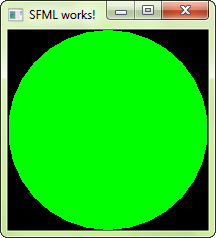
\includegraphics[scale=0.5]{../images/sfml_works.png}
\end{center}


\subsection*{Подключение вручную на Windows}
Если вы по какой-то причине не хотите использовать пакетные менеджеры (например, хотите установить другую версию библиотеки), то можно библиотеку подключить вручную. Для подключения библиотеки вам нужно сделать следующее:

\begin{enumerate}
\item Скачать нужную версию с сайта: \href{https://www.sfml-dev.org/}{sfml-dev.org}. Зайдите на этот сайт, нажмите на Downloads, а затем на Latest stable version, и выберите версию библиотеки, соответствующую вашему компилятору. Убедитесь, что версия полностью соответствует вашему компилятору, иначе библиотека не будет работать. В нашем курсе предполагается, что вы используете компилятор GCC MinGW 64-bit, но, возможно, вы используете другой компилятор.

\item Распакуйте скачанный архив. Он будет содержать папку с названием SFML и номер версии, например \texttt{SFML-2.6.1}. Переместите эту папку в удобное вам место на диске. Очень важно, чтобы путь до этой папки не содержал пробелы, кириллицу и какие-либо странные символы.

\item Зайдите в папку \texttt{SFML-<номер версии>}. В ней должны содержаться папки \texttt{bin}, \texttt{include}, \texttt{lib} и другие. Зайдите в папку \texttt{bin}, там должны лежать \texttt{.dll} файлы библиотеки SFML. Запомните название этой папки.

\item Добавьте в переменную среды \texttt{PATH} путь до папки, содержащей \texttt{.dll} файлы библиотеки SFML.

\item Если терминал был открыт, то закройте его, а потом откройте заново.
\end{enumerate}
Всё, библиотека установлена. Теперь можно компилировать файл исходного кода, использующий библиотеку SFML следующим образом:
\begin{verbatim}
  g++ main.cpp -I<путь до include> -L<путь до lib> -lsfml-graphics -lsfml-window -lsfml-system
\end{verbatim}
Например, если я переместил папку SFML просто на диск C и путь до этой папки это \texttt{C:\textbackslash SFML-2.6.1}, то нужная команда для компиляции будет:
\begin{verbatim}
  g++ main.cpp -I C:\SFML-2.6.1\include -L C:\SFML-2.6.1\lib -lsfml-graphics -lsfml-window -lsfml-system
\end{verbatim}
Это команда очень длинная, но вы можете вызвать её один раз. После этого можно нажимать клавишу вверх на клавиатуре, чтобы повторить команду. Или же можно просто где-то сохранить команду (в \texttt{.txt} файле на диске), а потом просто копировать её и вставлять в терминал.

\subsection*{Подключение вручную на Linux}
Этот способ совпадает со способом Windows, за исключением того, что вам не нужно устанавливать значение переменной \texttt{PATH}. Компилирование также совпадает:
\begin{verbatim}
  g++ main.cpp -I<путь до include> -L<путь до lib> -lsfml-graphics -lsfml-window -lsfml-system
\end{verbatim}

\subsection*{Использование \texttt{bat}-скрипта на Windows} 
Так как постоянно прописывать в терминале команду для компиляции может быть затруднительно, то можно положить весь процесс сборки в специальный \texttt{bat}-скрипт. \texttt{bat}-скрипт - это просто файл кода языка терминала Windows. Для того, чтобы использовать такой в файл в нашем случае нужно сделать следующее:
\begin{enumerate}
\item Cоздать в той папке, где лежит файл \texttt{main.cpp}, новый текстовый файл. 

\item Откройте этот новый текстовый файл и добавьте туда следующее:
\begin{verbatim}
  g++ %1 -I<путь до include> -L<путь до lib> -lsfml-graphics -lsfml-window -lsfml-system
  .\a.exe
\end{verbatim}
где вместо \texttt{<путь до include>} нужно подставить путь до \texttt{include} папки SFML, а вместо \texttt{<путь до lib>} -- путь до \texttt{lib} папки SFML. Сохраните и закройте файл.

\item Переименуйте этот текстовый файл в файл с расширением \texttt{.bat}. Например, в \texttt{run.bat}. Убедитесь, что ваша операционная система показывает расширения всех файлов и что файл действительно называется \texttt{run.bat}, а не, например, \texttt{run.bat.txt}.

\item Откройте терминал и в терминале зайдите в папку, содержащую файлы \texttt{main.cpp} и \texttt{run.bat}

\item Выполните в терминале команду
\begin{verbatim}
    run main.cpp
\end{verbatim}
или, если эта команда не сработала, то:
\begin{verbatim}
   .\run.bat main.cpp
\end{verbatim}
После этого всё содержимое файла \texttt{run.bat} исполнится (за место \texttt{\%1} подставится \texttt{main.cpp}), что означает, что ваша программа скомпилируется и запустится. То есть, теперь для компиляции и запуска программы достаточно написать в терминале одну команду \texttt{run}. Если понадобиться скомпилировать другую программу, то файл \texttt{run.bat} можно будет скопировать к этой программе.
\end{enumerate}

\iffalse
\subsection*{Использование \texttt{bash}-скрипта на Linux} 
Так как постоянно прописывать в терминале сборку проекта может быть затруднительно, то можно положить весь процесс сборки в специальный \texttt{bash}-скрипт. \texttt{bash}-скрипт - это просто файл кода языка терминала linux. Пример можно посмотреть в \texttt{2sfml/1bash\_script}.



\newpage
\subsection*{Подключение с помощью \texttt{cmake} (файл CMakeLists.txt)}
Система автоматической сборки \texttt{cmake} позволяет собирать большие проекты. Чтобы работать с ней вам нужно её скачать по адресу \href{https://cmake.org/}{cmake.org} и установить переменную среды \texttt{PATH}. Затем нужно создать файл \texttt{CMakeLists.txt} в директории вашего проекта и написать в нём:
\begin{verbatim}
cmake_minimum_required(VERSION 2.8.0)
project(simple_sfml)
 
# Создадим исполняемый файл по имени simple_sfml из исходного файла main.cpp
add_executable(simple_sfml main.cpp)

# Найдём библиотеку SFML автоматически с компонентами graphics, system и window
find_package(SFML 2.5 COMPONENTS graphics system window)
# Подключим эту библиотеку
target_link_libraries(simple_sfml sfml-graphics sfml-system sfml-window)
\end{verbatim}

После этого, проект можно собрать так:
\begin{verbatim}
cmake -G<генератор> <путь до CMakeLists.txt>
\end{verbatim}

Пример make-файла можно посмотреть в папке \texttt{classroom\_tasks/2sfml/4cmake} и\\ \texttt{classroom\_tasks/2sfml/5cmake\_find\_package}\\
\begin{itemize}
\item Соберите проект в папке \texttt{0basics}, используя один из приведённых выше способов (предпочтительно - make или cmake). 
\end{itemize}


\newpage
\subsection*{Работа с библиотекой:}
Документация и туториалы по библиотеке SFML можно найти на оффициальном сайте:\\ \texttt{https://www.sfml-dev.org/}{sfml-dev.org}. Пример простой программы, для работы с SFML в папке \texttt{1sfml\_basics}. \\
Основные классы SFML и их методы:
\begin{itemize}
\item[--] \texttt{sf::Vector3f, sf::Vector2f, sf::Vector2i} и т. д. Классы для математического вектора с перегруженными операциями. (аналогичные тем, что мы писали на предыдущих занятиях). \\
\href{https://www.sfml-dev.org/documentation/2.5.1/classsf_1_1Vector2.php}{sfml-dev.org/documentation/2.5.1/classsf\_1\_1Vector2.php}
\item[--] \texttt{sf::RenderWindow} - класс для окна.
\href{https://www.sfml-dev.org/documentation/2.5.1/classsf_1_1RenderWindow.php}{sfml-dev.org/documentation/2.5.1/classsf\_1\_1RenderWindow.php}
\item[--] \texttt{sf::CircleShape} - класс для фигуры - круг.
\href{https://www.sfml-dev.org/documentation/2.5.1/classsf_1_1CircleShape.php}{sfml-dev.org/documentation/2.5.1/classsf\_1\_1CircleShape.php}
\end{itemize}
\fi


\newpage
\section{Основные классы библиотеки SFML}
\subsubsection*{Типы целых чисел}
Так как библиотека SFML кросплатформенная, то в ней введены \texttt{typedef}-синонимы для целочисленных типов, например \texttt{Int8}, \texttt{Int64}, \texttt{Uint32} и другие. Эти типы гарантируют, что они будут соответствующего размера.

\subsubsection*{Классы математических векторов}
Классы двумерных математических векторов \texttt{sf::Vector2<T>}. У них есть два публичных поля: \texttt{x} и \texttt{y}. Также, для них перегруженны операции сложения с такими же векторами и умножения на числа. Также введены \texttt{typedef}-синонимы вроде \texttt{sf::Vector2f} для \texttt{sf::Vector2<float>} и другие.
\begin{lstlisting}
sf::Vector2f a {1.0, 2.0};
sf::Vector2f b {3.0, -1.0};

sf::Vector2f c = 2.0f * (a + b);
std::cout << c.x << " " << c.y << std::endl;  // Напечатает  8 2
\end{lstlisting}

\subsubsection*{Класс цвета}
Класс цвета \texttt{sf::Color}. Имеет 4 публичных поля: \texttt{r}, \texttt{g}, \texttt{b}, \texttt{a} - компоненты цвета в цветовой модели RGB и прозрачность. Есть конструктор от 3-х или 4-х аргументов. Есть перегруженные операции для сравнения и сложения цветов. Есть уже определённые цвета вроде \texttt{sf::Color::Blue} и другие.

\begin{lstlisting}
sf::Color a {100, 200, 50};
sf::Color b {100, 100, 0};

sf::Color c = a + b;
std::cout << c.r << " " << c.g << " " << c.b << std::endl;  // Напечатает 200 255 50
\end{lstlisting}



\subsubsection*{Класс времени}
Класс \texttt{sf::Time} для работы со временем. Есть методы \texttt{asSeconds}, \texttt{asMilliseconds} и \texttt{asMicroseconds}, которые возвращают время в виде числа в соответствующих единицах. Перегружены операторы сложения, умножения и другие. Есть дружественные функции \texttt{sf::seconds}, \texttt{sf::milliseconds} и \texttt{sf::microseconds}, которые принимают число, и возвращают соответствующие объект класса \texttt{sf::Time}. Функция \texttt{sf::sleep(sf::Time t)} -- ожидает время \texttt{t}.

\subsubsection*{Класс часов}
\texttt{sf::Clock} -- это маленький класс для измерения времени. У него есть:
\begin{itemize}
\item Конструктор по умолчанию, часы запускаются автоматически после создания.
\item Метод \texttt{getElapsedTime()} -- возвращает объект \texttt{sf::Time} -- время прошедшее с последнего запуска часов.
\item Метод \texttt{restart()} -- заново запускает часы и возвращает объект \texttt{sf::Time} -- время прошедшее с предыдущего запуска часов.
\end{itemize}

\begin{lstlisting}
sf::Clock clock;

sf::Time t1 = clock.restart();
sf::sleep(sf::seconds(2));
sf::Time t2 = clock.restart();
    
std::cout << (t2 - t1).asMilliseconds() << std::endl;  // Напечатает 2000
\end{lstlisting}


\subsubsection*{Класс окна}
Прежде чем начать рисовать, нужно создать окно, которое будет отображать то, что мы нарисовали. Для этого в SFML есть класс \texttt{sf::RenderWindow}. Вот его основные методы:
\begin{itemize}
\item \texttt{RenderWindow(sf::VideoMode m, const sf::String\& title, sf::Uint32 style, sf::ContextSettings\& s)}
Конструктрор, с двумя обязательными и двумя необязательными аргументами. Его аргументы:
\begin{itemize}
\item Видеорежим - определяет размер окна.
\item Заголовок окна
\item Стиль окна, необязательный аргумент, может принимать следующие значения:
\begin{itemize}
\item[-] \texttt{sf::Style::None}
\item[-] \texttt{sf::Style::Titlebar} -- окно с заголовком
\item[-] \texttt{sf::Style::Resize}  -- окно у которого можно менять размер
\item[-] \texttt{sf::Style::Close} -- окно с кнопочкой закрывания
\item[-] \texttt{sf::Style::Fullscreen} -- полноэкранный режим
\item[-] \texttt{sf::Style::Default = sf::Titlebar | sf::Resize | sf::Close} 
\end{itemize}
Этот параметр имеет значение по умолчанию (\texttt{sf::Default}).

\item Дополнительные настройки контекста OpenGL, необязательный аргумент.
\end{itemize}

\item \texttt{getPosition} и \texttt{setPosition} - получить или установить положение окна.
\item \texttt{getSize} и \texttt{setSize} - получить или установить размер окна в пикселях.
\item \texttt{setFramerateLimit} -- установить лимит для количества кадров в секунду.
\item \texttt{clear} - принимает цвет и очищает скрытый холст этим цветом
\item \texttt{draw} - рисует объект на скрытый холст
\item \texttt{display} - отображает на экран всё что было нарисовано на скрытом холсте
\end{itemize}


\subsubsection*{Классы фигур}
В SFML есть несколько классов для работы с простыми фигурами: \texttt{sf::CircleShape} (круг или элипс),\\ \texttt{sf::RectangleShape} (прямоугольник), \texttt{sf::ConvexShape} (фигура сложной формы, задаваемая точками). У этих классов есть общие методы:
\begin{itemize}
\item \texttt{setOrigin} - установить локальное начало координат фигуры. Положение этой точки задаётся относительно верхнего левого угла прямоугольника, ограничивающего фигуру. По умолчанию эта точка равна \texttt{(0, 0)}, то есть локальным началом координат фигуры считается её верхний левый угол.  Эта точка важна, так как относительно неё происходят все операции поворота и масштабирования.
\item \texttt{setPosition}, \texttt{getPosition} - задать и получить координаты фигуры. Фигура перемещается таким образом, чтобы её \texttt{origin} оказался в заданой точке.
\item \texttt{move} - принимает 2D вектор и передвигает фигуру на этот вектор.
\item \texttt{setRotation}, \texttt{getRotation} - задать и получить угол (в градусах) вращения фигуры вокруг точки \texttt{origin}
\item \texttt{rotate} - принимает вещественное число и вращает фигуру на этот угол (в градусах)
\item \texttt{setScale}, \texttt{getScale} - задать и получить величину масштабирования (2D вектор)
\item \texttt{scale} - принимает  2D вектор и растягивает или сжимает фигуру по x и по y соответственно
\item \texttt{setFillColor}, \texttt{getFillColor} -- устанавливает/возвращает цвет заливки фигуры
\end{itemize}


\subsection*{Простая программа, которая рисует движущийся круг}
\begin{lstlisting}
#include <SFML/Graphics.hpp>
int main()
{
    sf::RenderWindow window(sf::VideoMode(800, 800), "Moving Circle", sf::Style::Default);
    window.setFramerateLimit(60);
    
    sf::CircleShape circle(30);
    circle.setPosition(sf::Vector2f{100, 100});

    while (window.isOpen())
    {
        sf::Event event;
        while (window.pollEvent(event)) 
        {
            if (event.type == sf::Event::Closed)
                window.close();
        }
        circle.move(sf::Vector2f{1, 1});

        window.clear(sf::Color::Black);
        window.draw(circle);

        window.display();
    }
}
\end{lstlisting}
Пояснения по программе:

\begin{itemize}
\item В строке:
\begin{lstlisting}[frame=none]
sf::RenderWindow window(sf::VideoMode(800, 800), "Moving Circle", sf::Style::Default);
\end{lstlisting}
создаётся объект класса окна, устанавливается разрешение окна и названия окна, а также стиль окна.
\item В строке:
\begin{lstlisting}[frame=none]
window.setFramerateLimit(60);
\end{lstlisting}
Ограничивает максимальное количество кадров в секунду (англ. \textit{frames per second} или \textit{fps}) числом 60. Если не прописать эту строку, то на мощных компьютерах все движения в программе будут происходить быстрее, так как за секунду будет вполняться намного больше, чем 60 итерации главного цикла. Метод \texttt{setFramerateLimit} заставляет программу ожидать после каждого цикла, чтобы общее время одной итерации главного цикла была равна как минимум $1/60$ секунды.

Но нужно понимать, что этот метод ограничивает только максимальное количество fps. Если за один кадр выполняется много вычислений, то fps может просесть ниже 60. Из за этого все движения объектов в программе будет происходить медленнее. Чтобы скорость движения объектов не зависила от мощности компютера нужно высчитывать время, занятое на каждом кадре, и передвигать объект в соответствии с этим временем.


\item В строке:
\begin{lstlisting}[frame=none]
sf::CircleShape circle(30);
circle.setPosition(sf::Vector2f{100, 100});
\end{lstlisting}
создаём объект круга и устанавливаем его положение в точку с координатами \texttt{(100, 100)}. Учтите, что в SFML ось Y направлена сверху вних. То есть значение \texttt{y = 0} будет находится в самом верху экрана, а значение \texttt{y = 800} будет находиться в самом низу нашего экрана высотой 800 пикселей.


\item Дальше, со строки:
\begin{lstlisting}[frame=none]
while (window.isOpen())
\end{lstlisting}
начинается  \textit{главный цикл} программы. Каждая итерация этого цикла -- это один кадр прогаммы. Цикл заканчивается когда у объекта окна вызовется метод \texttt{close}.

\item В строках:
\begin{lstlisting}[frame=none]
sf::Event event;
while (window.pollEvent(event)) 
{
    if (event.type == sf::Event::Closed)
        window.close();
}
\end{lstlisting}
написан \textit{цикл обработки событий}. Событиями могут быть, например, нажатие клавиш или кнопок мыши, движение мыши, изменение размера экрана, закрытие окна. За время одного кадра может произойти несколько событий. Все эти события помещаются в специальную очередь. В начале каждой итерации главного цикла нужно взять из этой очереди все события и обработать их.

В данном простом цикле обработки событий, обрабатывается только событие закрытия окна (нажатие на красный крестик). При нажатии на красный крестик, программа будет закрываться.

\item В строке:
\begin{lstlisting}[frame=none]
circle.move(sf::Vector2f{1, 1});
\end{lstlisting}
мы передвигаем кружок на один пиксель вправо по оси X и на один пиксель вниз по оси Y.

\item В строке:
\begin{lstlisting}[frame=none]
window.clear(sf::Color::Black);
\end{lstlisting}
мы закрашиваем \textit{скрытый холст} черным цветом. Это нужно делать, чтобы закрасить то, что было нарисовано на предыдущем кадре. Скрытый холст -- это просто двумерный массив из цветов пикселей размера \texttt{ширина окна x высота окна}, находящийся в памяти компьютера. После закраски скрытого холста никаких изменений на экране не произойдёт, так как скрытый холст на экран не отображается. В это время на экран отображается содержимое \textit{первичного холста}.


\item В строке:
\begin{lstlisting}[frame=none]
window.draw(circle);
\end{lstlisting}
кружок рисуется на скрытый холст. Опять, никаких видимых изменений на экране не будет, так как на экран отображается первичный холст.

\item В строке:
\begin{lstlisting}[frame=none]
window.display();
\end{lstlisting}
скрытый и первичный холст меняются местами. Скрытый холст становится первичным, а первичный скрытым. Теперь всё, что мы нарисовали на скрытый холст станет видимым. Такой способ чередования холстов называется \textit{двойная буферизация}. Он обеспечивает плавность анимации и отсутствие мерцаний. Если бы двойной буферизации не было, то в какие-то моменты времени мы видели бы на экране частично отрисованное изображение кадра, а в какие-то моменты весь кадр. Это выглядело бы как мерцание всех рисуемых объектов.



\end{itemize}
\newpage
\subsubsection*{Anti-Aliasing}
\begin{multicols}{2}
\begin{center}
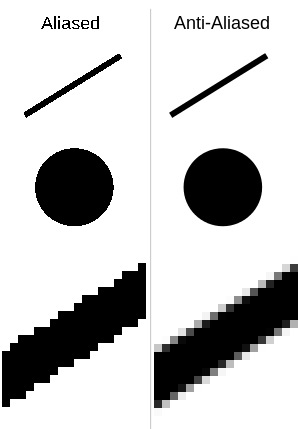
\includegraphics[scale=0.5]{../images/anti-aliasing.png}
\end{center}
Вы могли заметить, что фигуры выглядят не очень красиво - имеют зазубрены. Это связано с тем, что рисования происходит на прямоугольной сетке пикселей и при проведении линий под углом образуются ступеньки. Для борьбы с этим эффектом был придуман специальный метод сглаживания, который называется антиалиасинг. Он уже автоматически реализован во всех библиотеках компьютерной графики. Чтобы установить его в SFML, нужно прописать опцию:
\begin{lstlisting}
sf::ContextSettings settings;
settings.antialiasingLevel = 8;
\end{lstlisting}
И передать \texttt{settings} на вход для конструктора \texttt{RenderWindow}. Пример в папке \texttt{code/sfml\_basics}.
\end{multicols}


\subsubsection*{Класс строки}
В SFML есть свой класс строки под названием \texttt{sf::String}. Поддерживает разные виды кодировок. Имеет конструкторы от стандартных строк \texttt{C++} и строк в стиле \texttt{C}.


\subsubsection*{Класс шрифта}
Класс шрифта \texttt{sf::Font} нужен для загрузки данных шрифта с диска и использования этого шрифта при отрисовке текста. Файл шрифта можно найти в интернете, он имеет расширение \texttt{.ttf}. Загрузить шрифт в программу можно с помощью метода \texttt{loadFromFile} класса \texttt{sf::Font}:
\begin{lstlisting}
sf::Font font;
if (!font.loadFromFile("consola.ttf")) 
{
    std::cout << "Error. Can't load font!" << std::endl;
    std::exit(1);
}
\end{lstlisting}
Метод \texttt{loadFromFile} будет искать файл относительно исполняемого файла. То есть в примере выше нужно убедиться, что файл \texttt{consola.ttf} лежит в той же папке, что и исполняемый файл.

\subsubsection*{Класс текста}
\texttt{sf::Text} -- класс объекта для отображения текста на экране.
У объектов этого класса можно задать шрифт, содержимое строки, размер шрифта, цвет, стиль с помощью соответствующих методов. Положение текста на экране задаётся с помощью методов, аналогичных методам фигур: \texttt{setPosition}, \texttt{move}, \texttt{rotate} и других.


\newpage
\subsubsection*{Пример программы, которая рисует вращающийся текст}
\begin{lstlisting}
#include <SFML/Graphics.hpp>
#include <iostream>
int main()
{
    sf::RenderWindow window(sf::VideoMode(800, 800), "Rotating Text", sf::Style::Default);
    window.setFramerateLimit(60);
    
    sf::Font font;
    if (!font.loadFromFile("consola.ttf")) 
    {
        std::cout << "Error! Can't load font!" << std::endl;
        std::exit(1);
    }

    sf::Text text;
    text.setFont(font);
    text.setString(L"Привет");
    text.setCharacterSize(50);
    text.setFillColor(sf::Color(70, 160, 100));
    text.setStyle(sf::Text::Bold | sf::Text::Underlined);
    text.setPosition({300, 200});

    while (window.isOpen())
    {
        sf::Event event;
        while (window.pollEvent(event)) 
        {
            if (event.type == sf::Event::Closed)
                window.close();
        }
        text.rotate(0.1f);

        window.clear(sf::Color::Black);
        window.draw(text);

        window.display();
    }
}
\end{lstlisting}

\newpage
\subsubsection*{Опасность при использовании текста}
\begin{lstlisting}
#include <SFML/Graphics.hpp>

sf::Text getText(std::string fontFile)
{
	sf::Font font;
    if (!font.loadFromFile(fontFile))
    {
        std::cout << "Error! Can't load font!" << std::endl;
        std::exit(1);
    }
    
    sf::Text text;
    text.setFont(font);
    text.setString(L"Привет");
    text.setCharacterSize(50);
    text.setFillColor(sf::Color(70, 160, 100));
    text.setStyle(sf::Text::Bold | sf::Text::Underlined);
    text.setPosition({300, 200});
    return text;
}

int main()
{
    sf::RenderWindow window(sf::VideoMode(800, 800), "Rotating Text", sf::Style::Default);
    window.setFramerateLimit(60);
    
    sf::Text text = getText("consola.ttf");

    while (window.isOpen())
    {
        sf::Event event;
        while (window.pollEvent(event)) 
        {
            if (event.type == sf::Event::Closed)
                window.close();
        }
        text.rotate(0.1f);

        window.clear(sf::Color::Black);
        window.draw(text);

        window.display();
    }
}
\end{lstlisting}


\newpage
\section{Главный цикл}
Как правило, у любой программы, работающей на основе событийно-ориентированной модели, есть главный цикл. На каждой итерации данного цикла программа должна проделать все необходимые операции по подготовке и отрисовке следующего кадра. Число итераций этого цикла называется числом кадров в секунду (англ. frames per seconds - fps).

В папке \texttt{4mainloop} предсталена простейшая программа с главным циклом. Сейчас основной цикл программы работает без перерывов и, так как наша программа очень проста, то количество кадров в секунду может достигать огромных значений - больше 1000 fps. Мониторы не обновляют экран с такой скоростью и человеческий глаз тоже не способен воспринять такую частоту кадров. Поэтому не имеет смысла задавать fps очень высоким, его желательно ограничить. Это можно сделать с помощью метода \texttt{setFramerateLimit}. Пример в папке \texttt{06framerate\_limit}.

Этот метод ограничивает лишь максимальное количество кадров. Если за один кадр выполняется много вычислений, то fps может просесть ниже 60. Из за этого программы, которые завязанны на времени, могут работать некорректно. Например, в нашем примере скорость движения шарика зависит от числа кадров в секунду. Чтобы шарик двигался одинаково независимо от fps нужно высчитывать время, занятое на каждом кадре. Пример, как это делать в папке \texttt{07clock\_time}.



\subsection*{Проверка на нажатие клавиш и кнопок}
\subsubsection*{Класс клавиатуры}
Класс клавиатуры \texttt{sf::Keyboard}. Внутри этого класса, в публичной части, объявлен перечисляемый тип \texttt{Key}, в котором перечислены все клавиши. Например, чтобы проверить нажатие на пробел понадобится \texttt{sf::Keyboard::Space}. Название всех клавиш можно найти по следующей ссылке: \href{https://www.sfml-dev.org/documentation/2.5.1/classsf_1_1Keyboard.php}{Тут}.\\
У этого класса есть метод 
\begin{itemize}
\item \texttt{isKeyPressed} -- принимает клавишу и проверяет нажата ли она.
\end{itemize}
Пример -- в папке \texttt{08is\_key\_pressed}.


\subsubsection*{Класс мыши}
Класс мыши \texttt{sf::Mouse}. Внутри этого класса, в публичной части, объявлен перечисляемый тип \texttt{Button} в котором перечислены все кнопки мыши.
У этого класса есть метод:
\begin{itemize}
\item \texttt{isButtonPressed} принимает на вход \texttt{sf::Mouse::Button} и проверяет нажата ли соответствующая кнопка.
\item \texttt{getPosition()} -- возвращает положение мыши на в координатах всего экрана.
\item \texttt{setPosition(const sf::Vector2i\&)} --  устанавливает положение мыши на в координатах всего экрана
\item \texttt{getPosition(const sf::Window\&)} -- возвращает положение мыши на в координатах данного окна.
\item \texttt{setPosition(const sf::Vector2i\&, const sf::Window\&)} --  устанавливает положение мыши на в координатах данного окна.
\end{itemize}
Пример -- в папке \texttt{09is\_button\_pressed}.

\subsubsection*{Задачи:}
\begin{itemize}
\item Создайте 2 объекта: круг и квадрат. Круг должен двигаться при нажатии на стрелки. Квадрат должен двигаться при нажатии на \texttt{WASD}.
\item Сделайте так, чтобы при нажатии на левую кнопку мыши координаты круга становились бы равными координатам мыши.
\item Сделайте так, чтобы при нажатии на \texttt{Enter} цвет квадрата менялся случайным образом каждый кадр.
\item Сделайте так, чтобы квадрат передвигался вправо на 50 пикселей каждые 2 секунды. При этом, все остальное должно работать как прежде, то есть функцию \texttt{sf::sleep} использовать не получится.
\item Сделайте так, чтобы цвет круга плавно зависел от положения курсора на экране.

\item Создайте новый круг белого цвета и сделайте так, чтобы при наведении на него курсора, он становился красным.
\end{itemize}



\newpage

\section{События}
\begin{itemize}

\item \textbf{KeyPressed:} В папке \texttt{1key\_events} лежит пример программы, которая обрабатывает нажатия клавиш. Измените программу так, чтобы при нажатии на клавишу Enter кружок менял цвет на случайный.

\item \textbf{KeyReleased:} Измените программу так, чтобы при \textit{отпускании} клавиши пробел прямоугольник менял цвет на случайный (событие \texttt{sf::Event::KeyReleased}).

\item \textbf{MouseButtonPressed:} В папке \texttt{2mouse\_events} лежит пример программы, которая обрабатывает нажатия и движение мыши. Измените программу так, чтобы при нажатии на правую кнопку мыши, прямоугольник перемещался к положению мыши. Событие должно срабатывать только в момент нажатия, прямоугольник не должен двигаться при зажатии кнопки.
\begin{lstlisting}
if (event.type == sf::Event::MouseButtonPressed)
{
    if (event.mouseButton.button == sf::Mouse::Right)
    {
        std::cout << "the right button was pressed" << std::endl;
        std::cout << "mouse x: " << event.mouseButton.x << std::endl;
        std::cout << "mouse y: " << event.mouseButton.y << std::endl;
    }
}
\end{lstlisting}


\item \textbf{MouseMoved:} Событие, которое срабатывает тогда, когда двигается мышь.
\begin{lstlisting}
if (event.type == sf::Event::MouseMoved)
{
    std::cout << "new mouse x: " << event.mouseMove.x << std::endl;
    std::cout << "new mouse y: " << event.mouseMove.y << std::endl;
}
\end{lstlisting}
Измените программу так, чтобы прямоуголиник окрашивался в красный цвет тогда и только тогда, когда курсор мыши находится на прямоугольнике. Во всё остальное время прямоуголиник должен быть зелёным.

\item \textbf{Перетаскивание:} Создайте новый прямоугольник и сделайте его перетаскиваемым. При нажатии на него и последующим движении мыши он должен начать двигаться вместе с курсором. При отпускании мыши должен остаться на месте.



\end{itemize}

\newpage
\section{Задачи}
\begin{itemize}


\item \textbf{Вращающийся квадрат}
Создайте программу, которая будет рисовать на экране вращающийся квадрат.


\item \textbf{Движение по окружности}
Создайте программу, которая будет рисовать на экране круг, движущийся по окружности.

\item \textbf{Шарики:} В папке \texttt{collision\_circles} содержится заготовка кода. 
\begin{itemize}
\item Используйте этот код, чтобы найти пересечение двух шаров. Если в процессе движения шары начнут накладываются друг на друга, то они должны окрашиваться в красный цвет. После прекращения наложения, шары должны опять стать белыми. Для этого добавьте поле типа \texttt{sf::Color} в класс \texttt{Ball} и метод \texttt{bool is\_colliding(const Ball\& b) const}, который будет проверять 2 кружка на столкновение.
\item Измените программу так, чтобы кружки упруго отскакивали друг от друга. Для этого нужно, при столкновении шариков, обратить составляющую скорости параллельную прямой, соединяющую центры шариков.
\item Добавьте возможность добавления нового шарика по нажатию правой кнопки мыши.
\item Добавьте возможность стенки по нажатию левой кнопки мыши. Нужно зажать ЛКМ в одной точки и отпустить в другой, чтобы получить стенку. Стенка -- это просто отрезок. Но шарики должны от него должны отскакивать. Про обнаружение столкновений можно посмотреть в папке \texttt{collision\_examples}.
\end{itemize}


\item \textbf{Перетаскивание:} В папке \texttt{1draggable/} содержится заготовка исходного кода для этого задания. Эта программа просто рисует прямоугольник на экране. Сделайте его перетаскиваемым мышью. При нажатии на него и последующим движении мыши он должен начать двигаться вместе с курсором. При отпускании мыши должен остаться на месте.

\item \textbf{Класс \texttt{Draggable}:} Создайте класс \texttt{Draggable}, который будет описывать прямоугольник, который можно перетаскивать мышкой.


\item \textbf{Кнопка:} Создайте кнопку. Логика работы должна этой кнопки аналогичной логике работы обычной кнопки в ОС Windows:
\begin{itemize}
\item Кнопка представляет собой прямоугольник некоторого цвета и с текстом внутри.
\item Изначально кнопка имеет некоторый заданный цвет.
\item При наведении курсора мыши на кнопку, её цвет меняется.
\item При нажатии и зажатии левой кнопки мыши(ЛКМ) над кнопкой, её цвет меняется.
\item При отпускании ЛКМ, если курсор всё ещё находится на прямоугольнике, происходит некоторое действие (например, печать в консоль).
\item В иных случая действие не происходит (например, если мы зажали ЛКМ вне кнопки и отпустили над кнопкой, или если мы зажали ЛКМ над кнопкой и отпустили вне кнопки).
\end{itemize}

\item \textbf{Класс кнопки:}  Напишите класс \texttt{Button}, который будет описывать кнопку. 
\begin{itemize}
\item Создайте 1 круг. Сделайте так, чтобы при нажатии на кнопку цвет круга менялся бы на случайный.
\item Создайте 4 кнопки. Сделайте так, чтобы при нажатии на эти кнопки положение круга смещалось на 10 пикселей в одном из 4-х направлений (влево, вправо, вверх, вниз).
\end{itemize}
	
\item \textbf{Флажки:} Напишите класс \texttt{Checkbox}, который будет описывать флажок. Флажок должен включать в себя квадратик, на который можно нажимать и менять состояние флажка (вкл/выкл), а также текст рядом с этим квадратиком. Создайте несколько флажков и кнопку. При нажатии на кнопку в консоль должно печататься тексты всех включенных флажков.

\item \textbf{Контекстное меню:} Напишите класс \texttt{ContextMenu}, описывающий контекстное меню.
Создайте круг. И добавьте опции в контекстное меню так, чтобы можно было менять цвет и размер круга.
\end{itemize}




\end{document}